\documentclass{beamer}
\usepackage{amsmath}
\usepackage{icomma}
\usepackage[utf8]{inputenc}
\usepackage[T1]{fontenc}
\usepackage{polski}
\usepackage[polish]{babel}
\usepackage{hyperref}
\usepackage{float}
\usepackage{textcomp}
\usetheme{Darmstadt}
\usecolortheme{rose}

% Naprawa nazw z angielskiego
\def\figureautorefname{Rysunek}

%Strona streszczenia
\newenvironment{abstractpage}
  {\cleardoublepage\vspace*{\fill}\thispagestyle{empty}}
  {\vfill\cleardoublepage}
  
%Samo streszczenie
\newenvironment{abstractsection}[1]
  {\bigskip\selectlanguage{#1}%
   \begin{center}\bfseries\abstractname\end{center}}
  {\par\bigskip}

%Ładne ułamki w jednostkach fizycznych
\sisetup{per-mode=symbol}%

\beamertemplatenavigationsymbolsempty
\setbeamertemplate{footline}[frame number]

\begin{document}
	\section{Wprowadzenie}
	\begin{frame}
		\title[Omnivelma]{Symulacja dookólnej bazy mobilnej}
		\author{Radosław Świątkiewicz}
		\date{\today}
		\institute{Promotor: dr hab. inż. Wojciech Szynkiewicz \\ \footnotesize Instytut Automatyki i Informatyki Stosowanej \\ Wydział Elektroniki i Technik Informacyjnych \\ Politechnika Warszawska}
		\titlepage
	\end{frame}
	\begin{frame}
		\frametitle{Spis treści}
		\tableofcontents[currentsection]
	\end{frame}
	
	\section{Problem}
	\begin{frame}
		\frametitle{Platforma z P109}
		\begin{columns}[c]
			\column{0.5\textwidth}
			\centering
			\includegraphics[width=0.8\textwidth]{graphics/velma.png} \\
			Robot manipulacyjny Velma
			\column{0.5\textwidth}
			\centering
			\includegraphics[width=\textwidth]{graphics/omnivelma.png} \\
			Platforma na kołach Mecanum
		\end{columns}
	\end{frame}
	\begin{frame}
		\frametitle{Cel projektu --- zamodelowanie}
		Po co potrzebny jest model:
		\begin{itemize}
		 \item Pozwala bezpiecznie testować nowe oprogramowanie.
		 \item Przyspiesza budowanie algorytmów sterowania.
		 \item Ułatwia przeprowadzanie skomplikowanych i niemożliwych testów.
		 \item Daje możliwość implementacji nieistniejących czujników do testów.
		\end{itemize}
		Wymagania:
		\begin{itemize}
		 \item Reaguje na siły w podobny sposób, co robot.
		 \item Przyjmuje takie samo sterowanie.
		 \item Generuje odpowiednie dane z wirtualnych czujników.
		\end{itemize}
	\end{frame}
	
	\section{Platforma}
	\begin{frame}
		\frametitle{Koła Szwedzkie (Mecanum)}
		\centering
		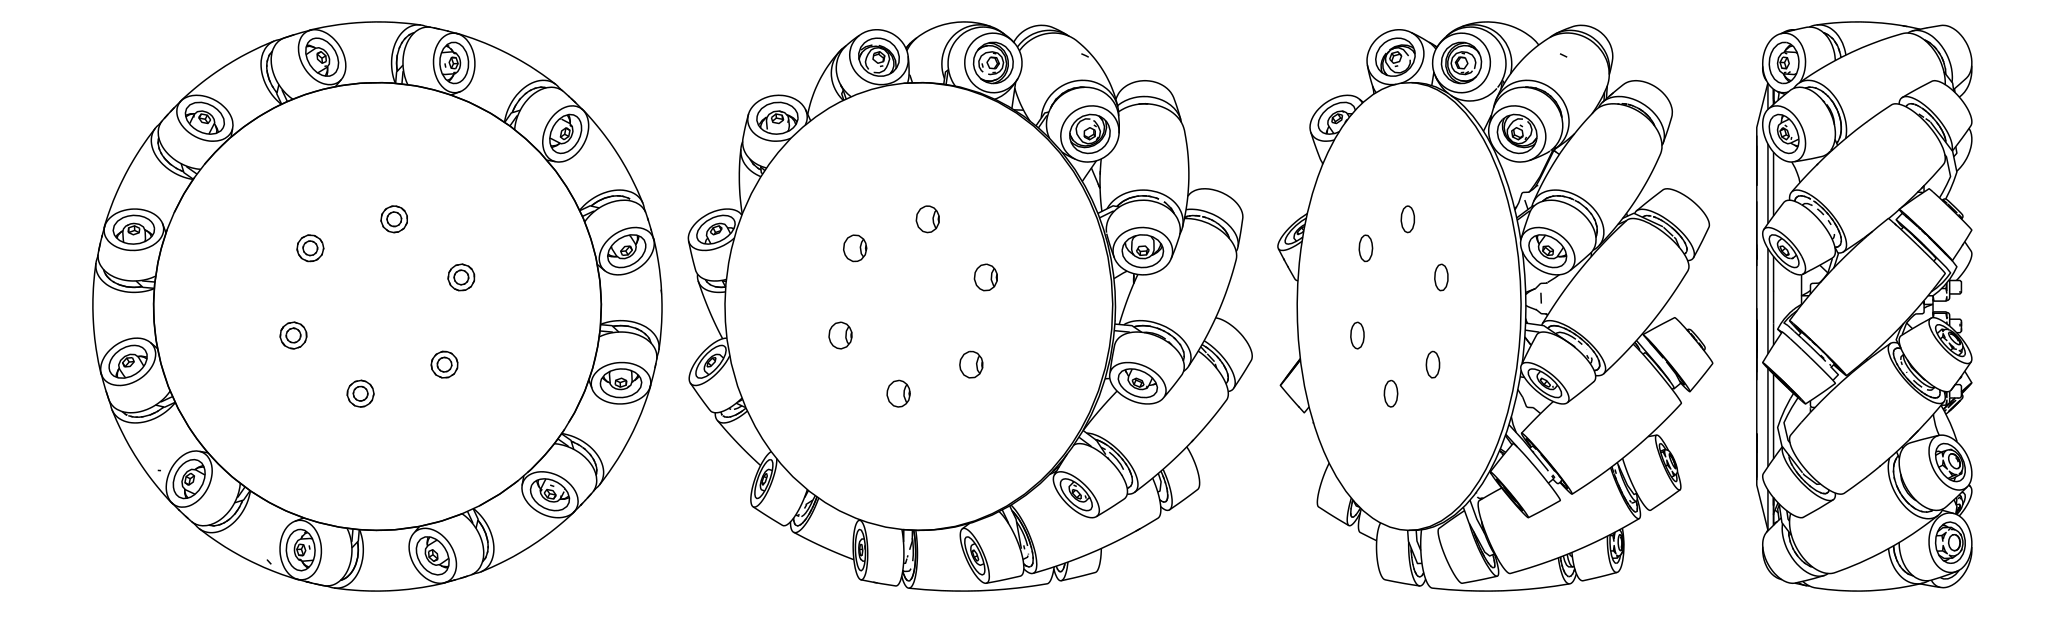
\includegraphics[width=\textwidth]{graphics/wheel.pdf}
		\begin{itemize}
			\item Każde koło ma 12 pasywnych rolek.
			\item Rolka obrócona względem osi o 45\textdegree.
			\item Punkt kontaktu powinien płynnie przechodzić z rolki na rolkę.
			\item Koło pod wpływem momentu siły i tarcia generuje dwa wektory zamiast jednego.
		\end{itemize}
	\end{frame}
	\begin{frame}
		\frametitle{Dodatkowy wektor}
		\centering
		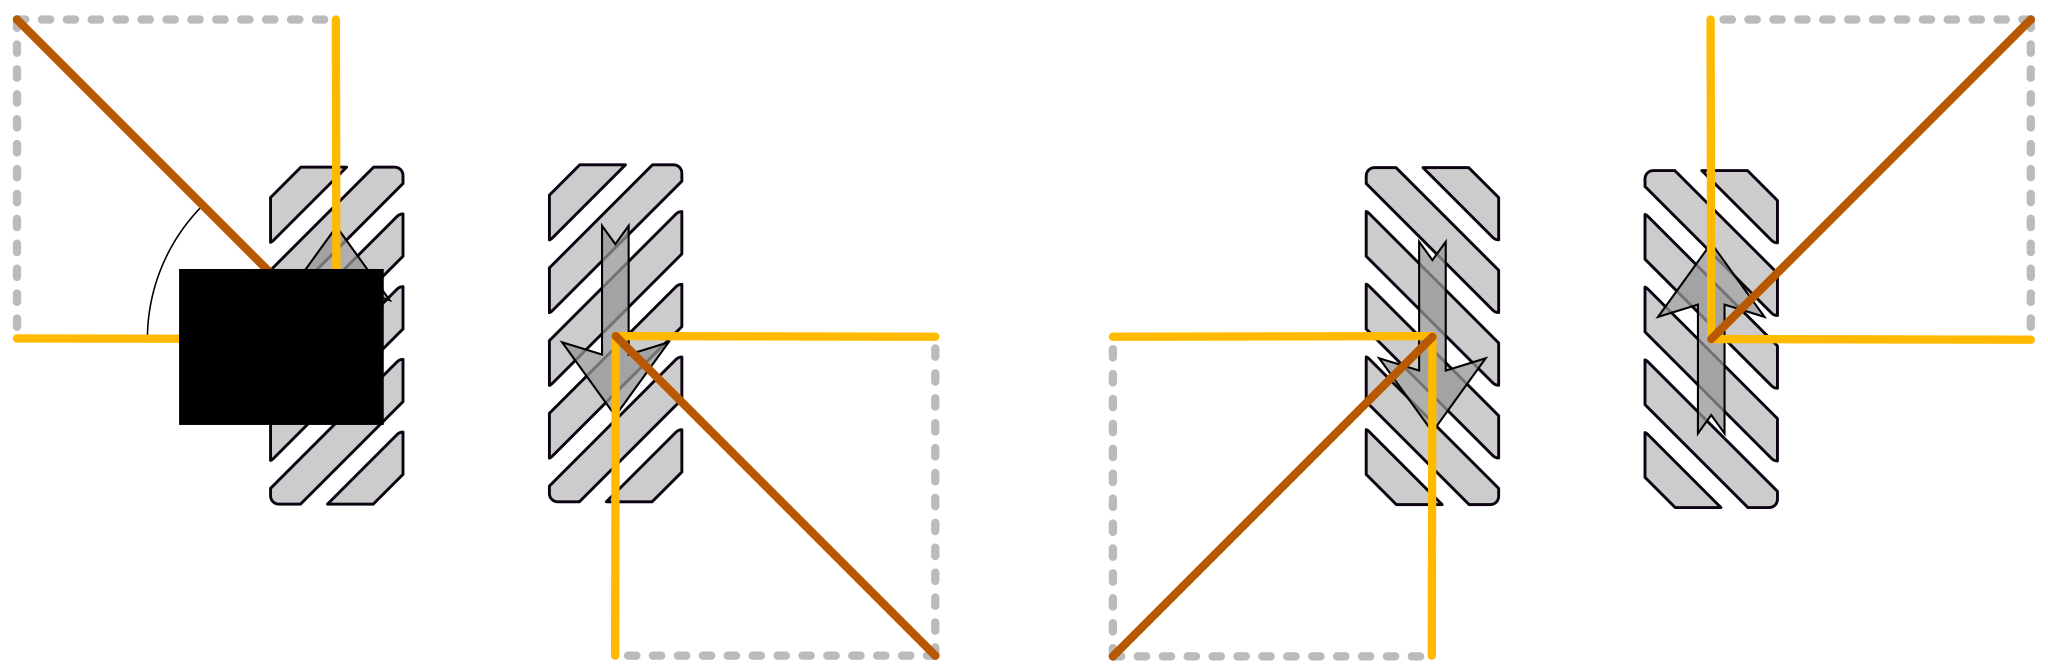
\includegraphics[width=\textwidth]{graphics/vectors.pdf} \\
		Standardowa opona pod wpływem tarcia przekształca prędkość kątową na liniową w płaszczyźnie obrotu.
		Koło Mecanum ma dodatkowy wektor równolegle do osi obrotu, zatem prędkość wypadkowa jest obrócona o 45\textdegree.
	\end{frame}
	\begin{frame}
		\frametitle{Kierunki ruchu}
		\centering
		\includegraphics[width=\textwidth]{graphics/dirs.pdf} \\
		Poprzez znoszenie się składowych prędkości, pojazd może poruszać się w kierunkach nieosiągalnych dla urządzeń o zwykłych kołach.
	\end{frame}
	\begin{frame}
		\frametitle{Kinematyka}
		Jak matematycznie przekształcić dane poszczególnych prędkości kół na wypadkową prędkość całości w danej chwili.
		\[
		\begin{bmatrix}
		v_x \\
		v_y \\
		\omega_z \\
		\end{bmatrix}
		=
		\frac{r}{4}
		\begin{bmatrix}
		-1 & 1 & -1 & 1 \\
		1 & 1 & 1 & 1 \\
		\frac{2}{a+b} & \frac{-2}{a+b} & \frac{-2}{a+b} & \frac{2}{a+b} \\
		\end{bmatrix}
		\begin{bmatrix}
		\omega_1 \\
		\omega_2 \\
		\omega_3 \\
		\omega_4 \\
		\end{bmatrix}
		\]
		\begin{table}
		\centering
		\begin{tabular}{c l}
		Oznaczenie & Opis \\
		\hline
		$r$ &  Promień koła w najszerszym miejscu. \\
		$a$ &  Szerokość platformy. \\
		$b$ &  Długość platformy. \\
		$\omega_i$ &  Prędkość kątowa kół. \\
		$v_x$ &  Prędkość transwersalna w osi X. \\
		$v_y$ &  Prędkość transwersalna w osi Y. \\
		$\omega_z$ &  Prędkość kątowa w osi Z (w górę). \\
		\end{tabular}
		\end{table}
	\end{frame}
	
	\section{Narzędzia}
	\begin{frame}
		\frametitle{Główne komponenty}
		\begin{columns}[c]
			\column{0.3\textwidth}
			\centering
			\includegraphics[width=\textwidth]{graphics/ros_logo.png} \\
			Logo ROS\footnotemark[1]
			\column{0.3\textwidth}
			\centering
			\includegraphics[width=\textwidth]{graphics/gazebo_logo.png} \\
			Logo Gazebo\footnotemark[2]
			\column{0.3\textwidth}
			\centering
			\includegraphics[width=\textwidth]{graphics/vrep_logo.png} \\
			Logo V-Rep\footnotemark[3]
		\end{columns}
		\footnotetext[1]{http://www.ros.org/}
		\footnotetext[2]{http://gazebosim.org/}
		\footnotetext[3]{http://www.v-rep.eu}
	\end{frame}

	\begin{frame}
		\frametitle{Struktura projektu}
		\begin{itemize}
			\item Symulator, który wczytuje model platformy i wystawia interfejs kolejek wiadomości ROS-a.
			\item Zbiór pakietów i narzędzi ROS-a pozwala na sprawne zarządzanie kolejkami.
			\item Program do manualnego sterowania robotem lub algorytm wyznaczania trasy.
			\item Programy zbierające dane do wyświetlenia.
		\end{itemize}
	\end{frame}
	
	\section{Implementacja}
	\begin{frame}
		\frametitle{Modele}
		\begin{columns}[c]
			\column{0.4\textwidth}
			\centering
			\includegraphics[width=\textwidth]{graphics/model.png} \\
			Dynamiczny model platformy.
			\column{0.6\textwidth}
			\begin{itemize}
				\item Model dynamiczny w Gazebo.
				\item Matematycznie doskonały model kinematyczny.
				\item Model dynamiczny w V-Repie.
			\end{itemize}
		\end{columns}
	\end{frame}
	
	\begin{frame}
		\frametitle{Manualne sterowanie}
		\begin{columns}[c]
			\column{0.5\textwidth}
			\centering
			\includegraphics[width=\textwidth]{graphics/lalkarz_1.png} \\
			\column{0.5\textwidth}
			\centering
			\includegraphics[width=\textwidth]{graphics/lalkarz_2.png} \\
		\end{columns}
		\begin{itemize}
			\item Generuje bezpośrednie zadane prędkości kół lub kierunek.
			\item Obsługuje wejście z klawiatury, kontrolera i myszki.
			\item Wyświetla wartości modelu czujnika enkoderów.
		\end{itemize}
	\end{frame}
	
	\section{Pomiary}
	\begin{frame}
		\frametitle{Obszar testów}
		\begin{columns}[c]
			\column{0.5\textwidth}
			\centering
			\includegraphics[width=\textwidth]{graphics/testfloor.png} \\
			Rysunki na podłożu do łatwego testowania.
			\column{0.5\textwidth}
			\centering
			\includegraphics[width=\textwidth]{graphics/track_1.png} \\
			Najprostszy przebieg po pierwszej trasie, bez obrotu wokół osi.
		\end{columns}
	\end{frame}
	\begin{frame}
		\frametitle{Powtarzalność}
		\begin{columns}[c]
			\column{0.5\textwidth}
			\centering
			\includegraphics[width=\textwidth]{graphics/bag_2.png} \\
			Druga trasa sterowana nieostrożnie.
			\column{0.5\textwidth}
			\centering
			\includegraphics[width=\textwidth]{graphics/bag_3.png} \\
			Trzecia trasa sterowana binarnie.
		\end{columns}
	\end{frame}
	\begin{frame}
		\frametitle{Pokaz?}
		Pokaz na żywo, bądź film.
	\end{frame}
 
	
	\section{Podsumowanie}
	\begin{frame}
		\frametitle{Aktualny stan}
		\begin{itemize}
			\item Eksperymenty są powtarzalne.
			\item Pomimo różnej budowy symulatorów i modeli, trasy są podobne.
			\item Istnieje wiele aspektów w których można próbować ulepszyć model.
		\end{itemize}
	\end{frame}
 
	\begin{frame}
		\frametitle{Ku przyszłości}
		\begin{itemize}
			\item Zdjęcie sterowania i przybliżonej trasy robota, a następnie ulepszanie modelu, aby jak najbardziej zbliżyć się do rzeczywistego przebiegu.
			\item Modyfikacje programu sterującego dla wygody.
			\item Próba implementacji modelu czujnika laserowego.
			\item Możliwie jak najbardziej dogłębna analiza modelu i określenie przyczyn rozbieżności.
		\end{itemize}
	\end{frame}
\end{document}